\begin{figure}
    \centering
    \begin{subfigure}[t]{0.3\textwidth}
         \centering
         \caption{}
         % \includesvg[pretex=\tiny, width=\textwidth]{../Figures/working/F1_ParadigmPredictions/chromaticity231109.svg}
         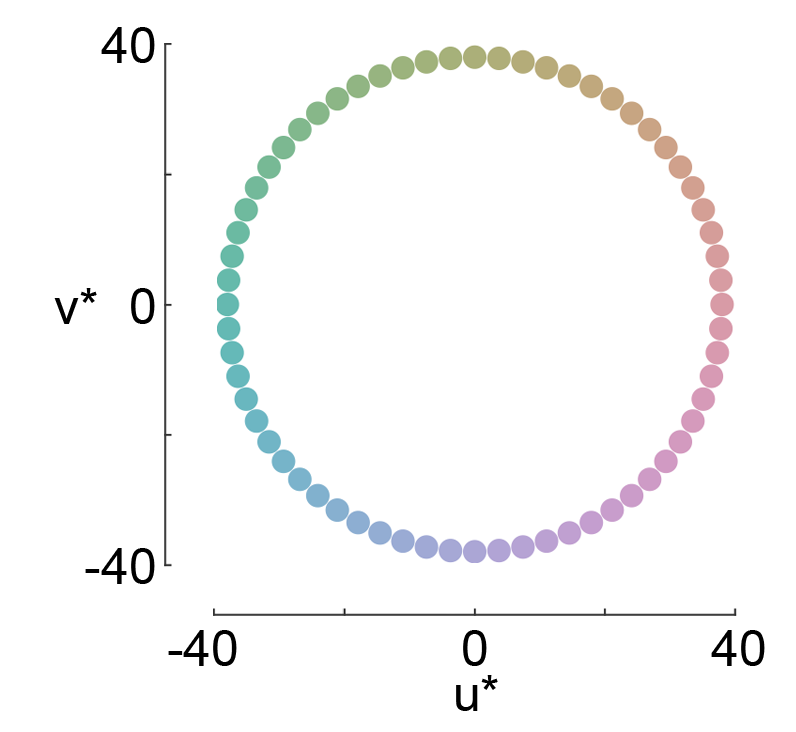
\includegraphics[width=\textwidth]{../Figures/working/F1_ParadigmPredictions/a.png}
         \label{fig:StimuliChromaticities}
    \end{subfigure}
    \hfill
    \begin{subfigure}[t]{0.65\textwidth}
         \centering
         \caption{}
         % \includesvg[pretex=\tiny, width=\textwidth]{../Figures/working/F1_ParadigmPredictions/epochs230620.svg}
        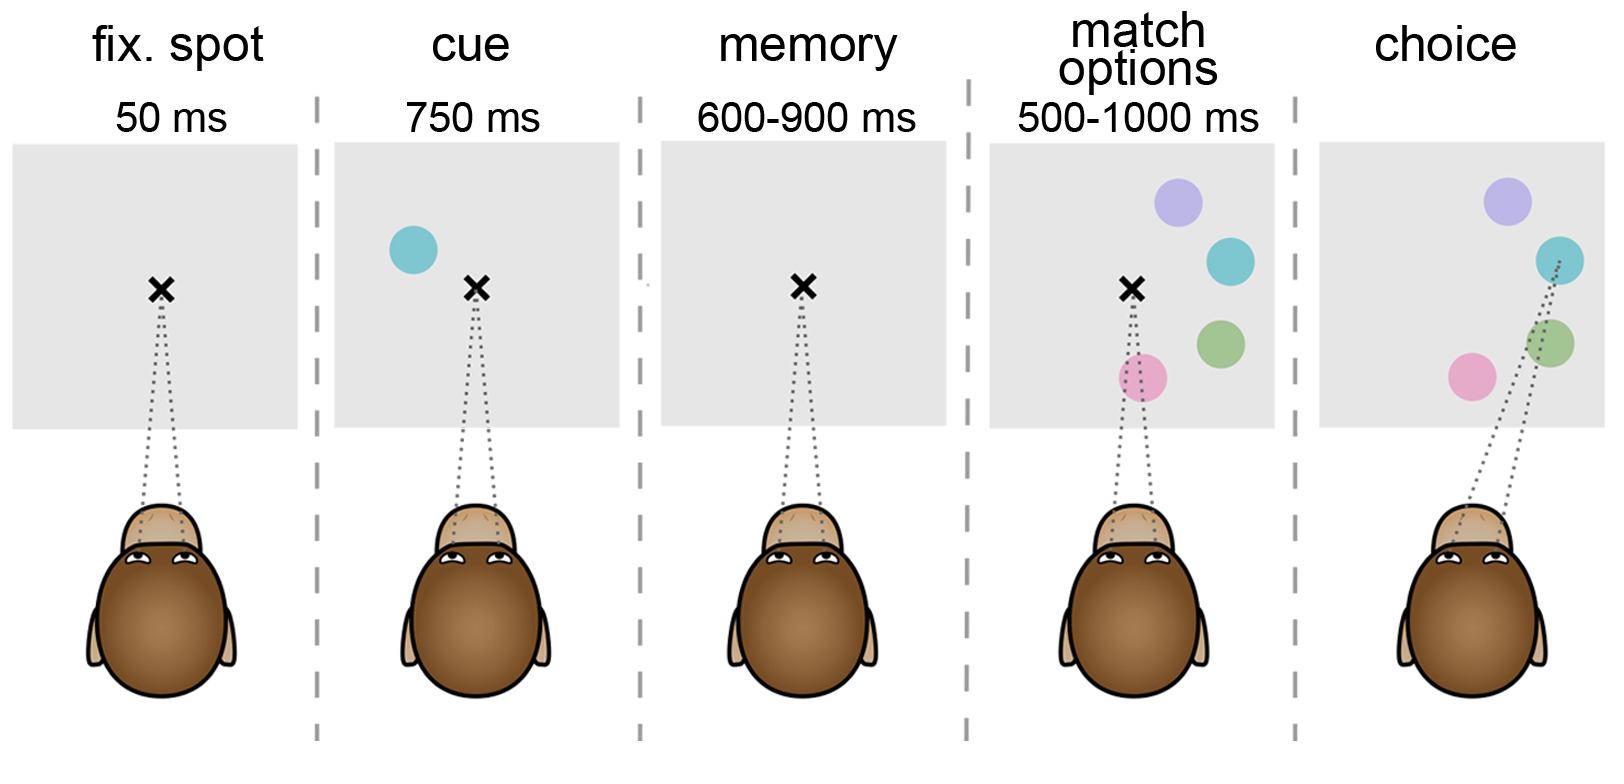
\includegraphics[width=\textwidth]{../Figures/working/F1_ParadigmPredictions/b.png}
         \label{fig:epochs}
    \end{subfigure}

    \begin{subfigure}[t]{0.45\textwidth}
         \centering
         \caption{}
         % \includesvg[pretex=\tiny, width=\textwidth]{../Figures/working/F1_ParadigmPredictions/bias1-230620.svg}
        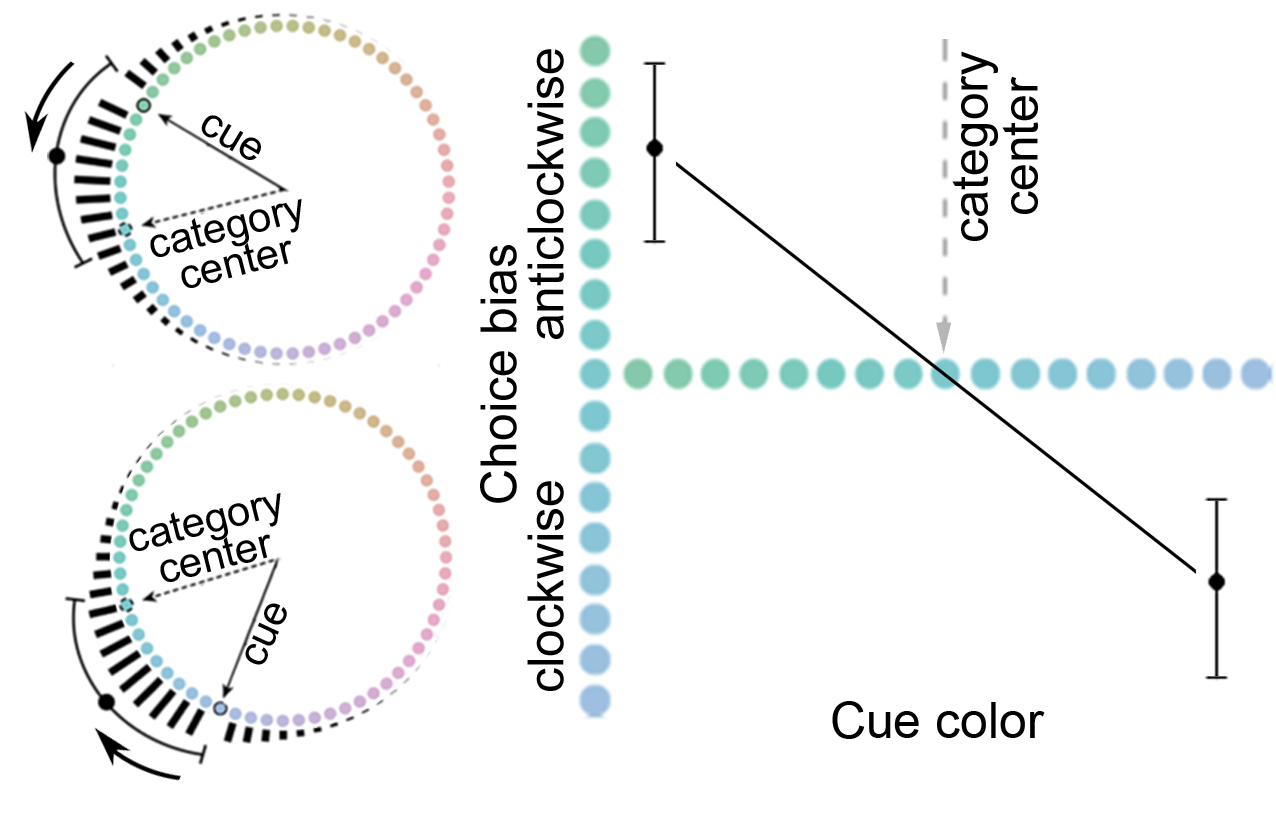
\includegraphics[width=\textwidth]{../Figures/working/F1_ParadigmPredictions/c.png}
         \label{fig:Bias1}
    \end{subfigure}
    %     \hfill
    % \begin{subfigure}[t]{0.20\textwidth}
    %      \centering
    %      \caption{}
    %      % \includesvg[pretex=\tiny, width=\textwidth]{../Figures/working/F1_ParadigmPredictions/bias2-230620.svg}
    %      \label{fig:Bias2}
    % \end{subfigure}
    % \hfill
    % \begin{subfigure}[t]{0.20\textwidth}
    %      \centering
    %      \caption{}
    %      \includegraphics[width=\textwidth]{example-image-a}
    %      \label{fig:BiasLinear}
    % \end{subfigure}
    \hfill
    \begin{subfigure}[t]{0.45\textwidth}
         \centering
         \caption{}
         % \includegraphics[width=\textwidth]{example-image-a}
        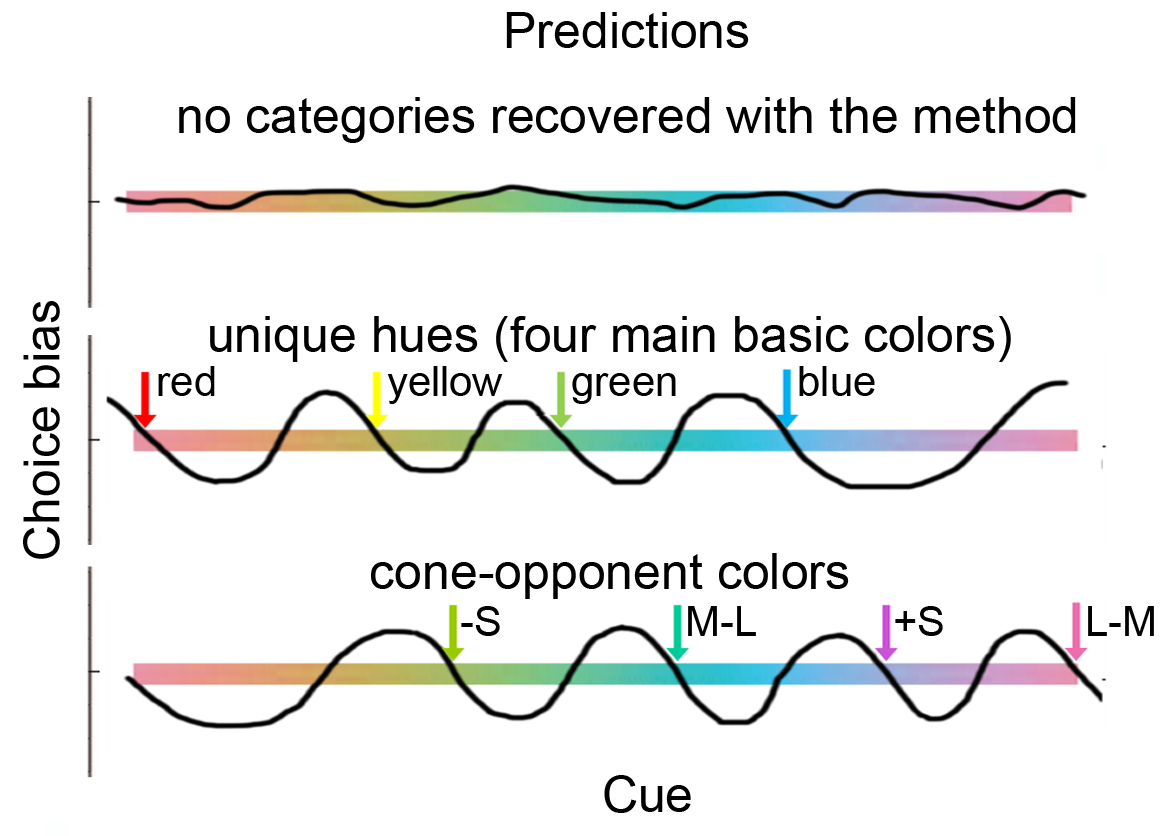
\includegraphics[width=\textwidth]{../Figures/working/F1_ParadigmPredictions/d.png}
         \label{fig:BiasPredictions}
    \end{subfigure}

    % 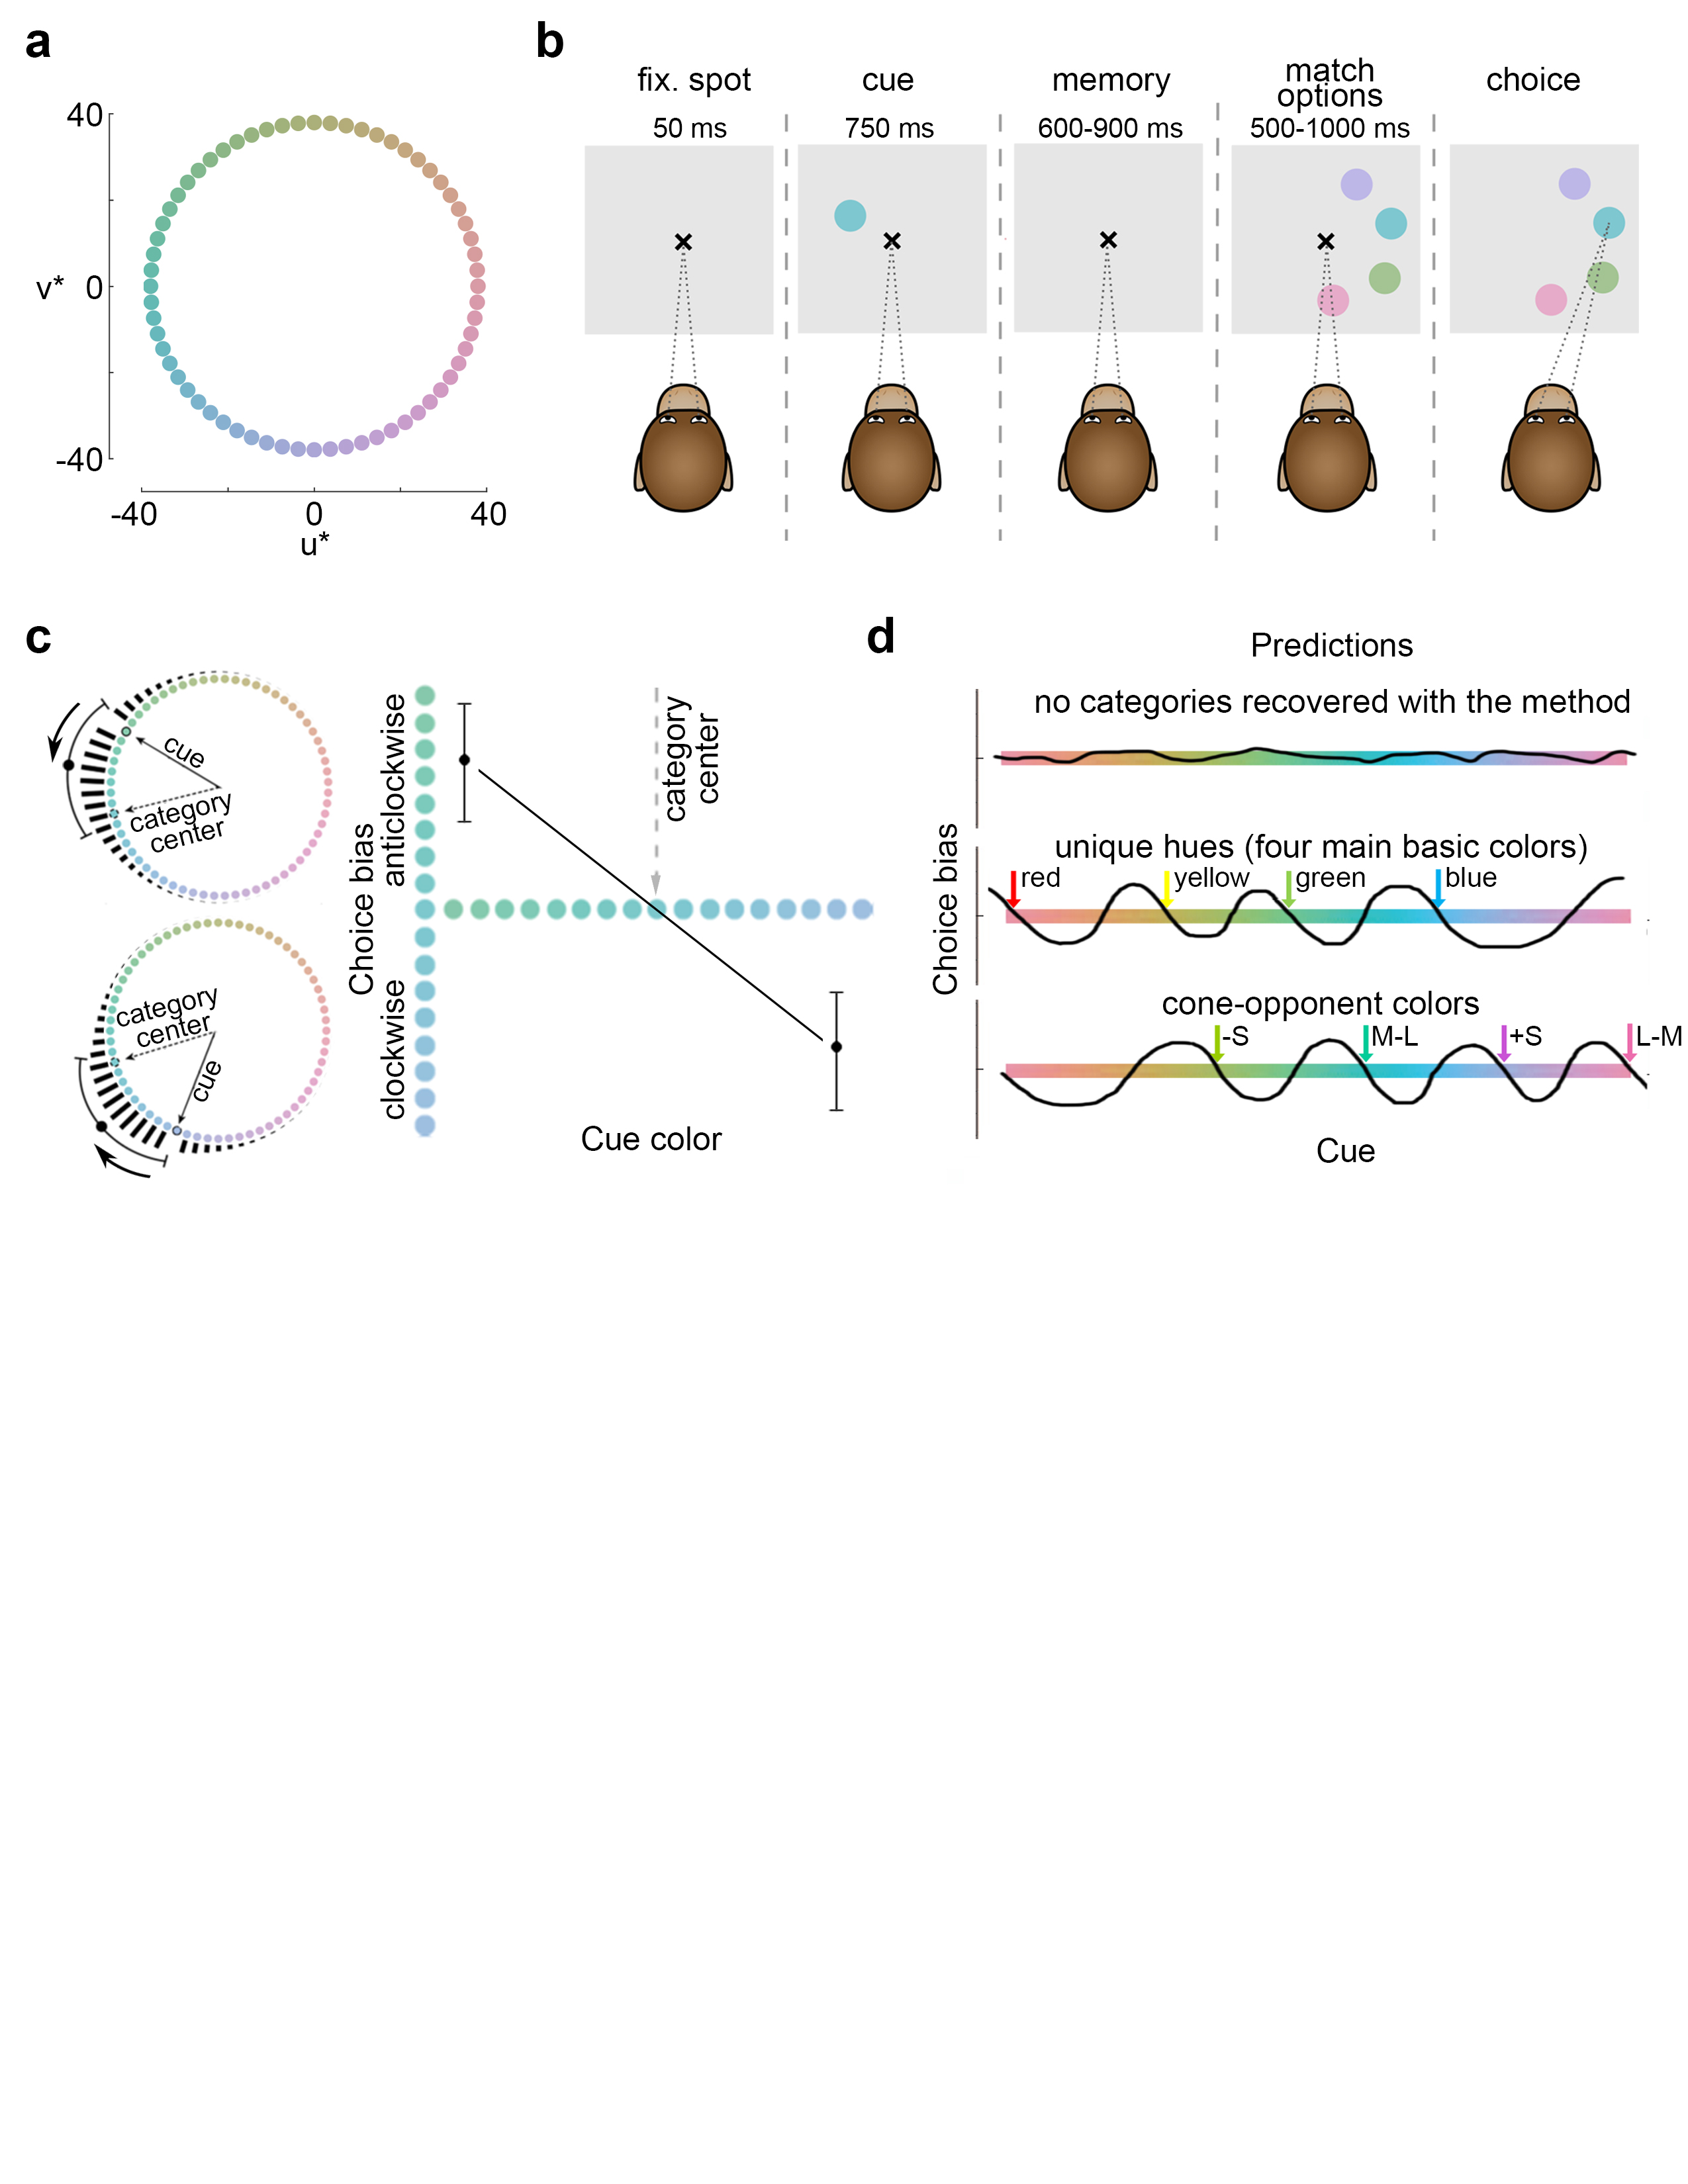
\includegraphics[width=\textwidth,trim={0 12cm 0 0},clip]{../Figures/flat/F1_ParadigmPredictions_3.jpg}
    
    \caption{\textbf{Non-verbal paradigm to recover color categories in non-human primates.}
    \emph{a}, Colors defined in CIELUV color space. \textbf{b}, Animals were trained to initiate a trial by fixating a small cross on a computer monitor and to maintain fixation throughout the trial until the fixation cross disappeared, which was their instruction to make a choice; trials in which the animals broke fixation were aborted. A 3-degree diameter cue was presented within the central 2.5 – 6-degrees, followed by a variable memory delay (600-900ms) and the presentation of the choice options. To mitigate impulsive choices, the choice options were shown for a variable amount of time (500-1000 ms) during which the animals needed to maintain fixation to avoid aborting the trial. After the fixation cross disappeared, the animals were free to make their selection. c, Predicted distribution of choices for two cues if a color category exists at the specified location in the color space (dashed arrow). The average of the distribution of choices will be shifted counterclockwise from the cue if the cue is displaced clockwise to the category center (top) and shifted clockwise from the cue if the cue is displaced counterclockwise to the category center (bottom). This pattern of results would be captured as the zero-crossing of the negative slope in a plot of the choice bias versus cue color (right). d, Predicted pattern of results for three hypotheses: no categories (top); the four most prominent basic color categories (also called the unique hues, middle); and the colors corresponding to the cone-opponent retinal encoding mechanisms (bottom). e, Data obtained in prior work on a related task in human subjects (see SI Figure 1 for three other data sets in human subjects, showing consistent pattern of results). Category centers seem to exist for colors that would be labeled in English as orange, green, blue, and purple. In the polar plot, the negative slopes demarking category centers are recovered by tracing the line in a counterclockwise direction, at points where it crosses the dashed circle marking zero choice bias. Repeller points (zero crossings of positive slope) appear to align with the -S, +S, and M-L poles of the cone-opponent axes (solid arrowheads), but not the L-M pole (open arrowhead).  
} 
    \label{fig:ParadigmAnalysisPredictions}
    
\end{figure}

Color categories are identified by color terms, of which the Basic Color Terms are considered prominent \citep{berlin_basic_1969}.
One hypothesis is that some subset of these terms are universal \citep{heider_universals_1972,regier_focal_2005}
and endowed by hard-wired neural mechanisms present at birth \citep{bornstein_categories_1976,lindsey_universality_2006}. 
This idea, put forth 150 years ago \citep{hering_zur_1875}, predicts some of the consistencies observed in color naming patterns across cultures \citep{jameson_evolutionary_2009,baronchelli_modeling_2010,lindsey_hunter-gatherer_2015,abbott_focal_2016}
and is consistent with some neurophysiological results \citep{clifford_electrophysiological_2009,holmes_neurophysiological_2009,brouwer_categorical_2013,bird_categorical_2014,yang_cortical_2016,forder_colour_2017}. 
Behavioral work in infants provides evidence for a biological origin of color categories \citep{franklin_new_2004,ozturk_language_2013}, but suggests that the innate categories are defined by retinal cone-opponent mechanisms rather than basic colors \citep{skelton_biological_2017,maule_color_2019}.
The infants in these experiments are typically several months old, by which stage they have had substantial cultural exposure, so evidence for color categories cannot conclusively be ascribed an innate origin.
Another hypothesis is that color categories emerge in development, instructed by language and culture \citep{roberson_color_2005, regier_language_2009, cibelli_sapir-whorf_2016}, and possibly involving an interplay of innate and developmental factors \citep{kay_language_2006,franklin_lateralization_2008,regier_language_2009}. 
This hypothesis is promoted by variability in color naming patterns across languages and individuals \citep{davidoff_colour_1999,roberson_color_2000,paramei_online_2018,webster_variations_2002}.
Current consensus is that some aspect of adult color category behavior is acquired through experience; the extent to which color categories are innate remains unresolved \citep{davidoff_nature_2009,skelton_colour_2023}.

An alternative approach to the origin of color categories could be provided by studying trichromatic non-human primates\citep{siuda-krzywicka_biological_2019}. 
The few studies on this topic have come to different conclusions: one found color categories in macaque monkeys seemingly consistent with categories in human adults \citep{sandell_color_1979}. 
This study inadvertently made comparisons substantially easier for cross-category than within-category trials, undermining its conclusion \citep{davidoff_cross-species_2010}. 
A later study tested for the existence of color categories across a limited range of colors and found a blue-green boundary in humans but not baboons \citep{fagot_cross-species_2006}.
The lack of color categories in the non-human primates could simply reflect the limited survey of color space. 
A third study, designed to investigate visual working memory, had two animals match color samples to a continuous ring of colors \citep{panichello_error-correcting_2019}. 
The experimental design is useful for studying visual working memory but complicates interpretation regarding color categorization because the animals could have been rewarded for making inaccurate matches, which would reinforce idiosyncratic biases, and indeed the two animals showed different patterns of behavior.

\paragraph{Measuring color categories in macaque monkeys}

Addressing the question of color categories in monkeys requires overcoming several challenges. 
First, how to measure color categories without teaching the animals the categories or reinforcing idiosyncratic biases \citep{essock_color_1977,matsuno_color_2004}.
Second, how to specify the color stimuli \citep{siuda-krzywicka_biological_2019}; for example, specifying the colors as wavelengths \citep{sandell_color_1979}
is not appropriate \citep{davidoff_cross-species_2010}. 
Third, how to obtain precise data across the full circle of hues so as to avoid missing categories \citep{fagot_cross-species_2006}.
A match-to-sample paradigm using colors defined in a perceptually uniform color space (\autoref{fig:StimuliChromaticities}) provides a potential solution to these challenges \citep{bae_why_2015}.
In the standard paradigm, a person is shown a color and asked to match the color to a continuous ring of colors, which is satisfactory for use in human participants who can follow instructions but introduces complications for use in monkeys.
So, we adapted the paradigm as an alternative-forced-choice task in which a direct match to the cue was available in every trial and the monkeys were only rewarded for making the direct match (\autoref{fig:epochs}). 
This task ensures precision in the matched colors and avoids the possibility of reinforcing biases acquired while the animals perform the task.
One consequence of this adapted paradigm is that it requires considerable data to sample category performance across the space of colors. 
Four animals performed the task, completing a total of 209456 trials over 232 sessions (see \autoref{fig:Indi_difficulty}).

\begin{figure}
    \centering
        \begin{subfigure}[t]{0.36\textwidth}
         \centering
         \caption{}
         \includesvg[pretex=\ttiny,width=\textwidth]{../Figures/working/F2_CombinedMMResults/difficulty_combinedData231110-004913.svg}
         \label{fig:CombinedDifficulty}
    \end{subfigure}
    \hfill
    \begin{subfigure}[t]{0.36\textwidth}
         \centering
         \caption{}
         \includesvg[pretex=\ttiny, width=\textwidth]{../Figures/working/F2_CombinedMMResults/F2_CombinedMMResults_fromModelOutput_MixMod_linear_231110-001902.svg}
         \label{fig:CombinedLinear}
    \end{subfigure}
    \hfill
    \begin{subfigure}[t]{0.25\textwidth}
         \centering
         \caption{}
         \includesvg[pretex=\ttiny, width=\textwidth]{../Figures/working/F2_CombinedMMResults/F2_CombinedMMResults_fromModelOutput_MixMod_polar_231110-001903.svg}
         \label{fig:CombinedPolar}
    \end{subfigure}
    \caption{\textbf{Task performance, and bias as a function of hue.}
    \emph{A.} Accuracy as a function of difficulty (where we define difficulty as the angular chromatic distance between the cue color and the closest incorrect choice option).
    \emph{B.} Bias as a function of hue (filled colored circles), smoothed (black line), with 95\% confidence intervals (grey filled area) and nominal categories highlighted by colored vertical stripes (where the width describes the 90\% confidence interval). The nominal categories occur at zero-crossing with negative slope.
    \emph{B.} As \autoref{fig:CombinedLinear} but in polar coordinates.
    }
    \label{fig:AvResults}
\end{figure}

If a monkey has a color category, the category center will be an attractor in the color space, captured by a zero-crossing of negative slope in a plot of the choice bias (\autoref{fig:Bias1}). 
Repellor points would be captured by the zero-crossing of the positive slope.
The approach is data-driven so it will recover whatever categories exist; nonetheless, before collecting the data we considered three possibilities. 
First, that the monkeys would show no color categories, as predicted by the work sampling a limited range of colors in baboons \citep{davidoff_cross-species_2010}
(\autoref{fig:BiasPredictions}, top);
second, that macaque color categories would correspond to  four main basic color categories as predicted by data in human adults (\autoref{fig:BiasPredictions}, middle); 
and third, that macaque color categories would align with repellants marked by the cone-opponent mechanisms as predicted by data in human infants \citep{skelton_biological_2017} (\autoref{fig:BiasPredictions}, bottom). 
Results in human participants, across multiple variants of the color-matching task in studies from different groups, clearly show evidence for four categories \citep{bae_why_2015,panichello_error-correcting_2019}, matching the number of categories stipulated in the second and third hypotheses but not clearly distinguishing them (\autoref{fig:humanData}; \autoref{fig:SIhumanData}) — the categories correspond to green, blue, orange, and pink. 
One possibility raised by the prior literature is that these differ from the canonical set of four basic colors (green, blue, yellow, red) because of limitations imposed by ensuring equal saturation and luminance among the colors (see \citep{bae_why_2015}). 

In the present experiments, the four animals performed well on the task, achieving a lapse rate if 7\%, 7.1\%, 5.8\%, 14.3\% (\autoref{fig:CombinedDifficulty}; the average performance across animals along with plots of individual animals showing 95\% CI are provided in \autoref{fig:Indi_difficulty}). % Currently there's only the individual in the SI, not the combined !!!!!!
The results provided clear evidence of choice biases in all four animals (\autoref{fig:AvResults}).
But the inferred color categories, averaged across the four animals, do not support any of the predictions (\autoref{fig:AvResults}): the animals appeared to show two consensus color categories,not four as in humans. 
To the extent that the macaque is an accurate model of the human, these results show that the four color categories manifest in humans are not innate. 
The two category centers recovered in the monkeys, at angle 13 (a peach color) and 211 (a teal color), were not  aligned with either of the cone-opponent mechanisms (arrowheads, \autoref{fig:CombinedPolar}); data for individual animals is shown in \autoref{fig:BiasCurvesIndividual}).

\paragraph{Two possible explanations for choice biases in macaque monkeys}

\begin{figure}
    \centering

    \begin{subfigure}[t]{0.3\textwidth}
         \centering
         \caption{}
       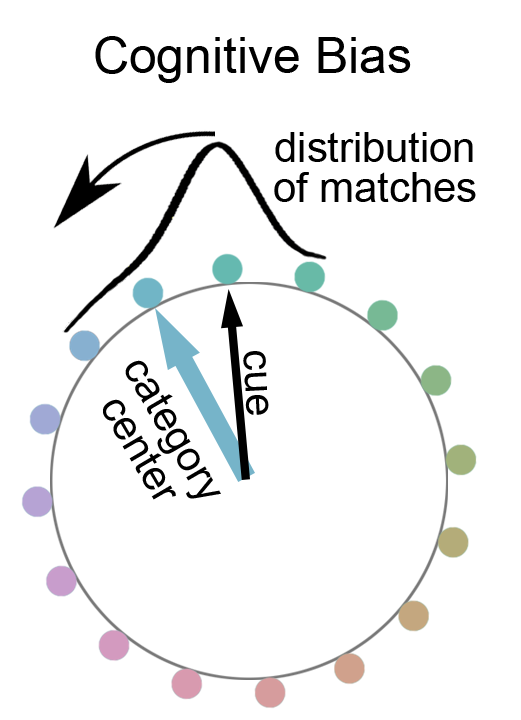
\includegraphics[height=4cm]{../Figures/working/F3_TCCModel/a.png}
         \label{fig:TCCCartoonA}
    \end{subfigure}
    \begin{subfigure}[t]{0.3\textwidth}
         \centering
         \caption{}
       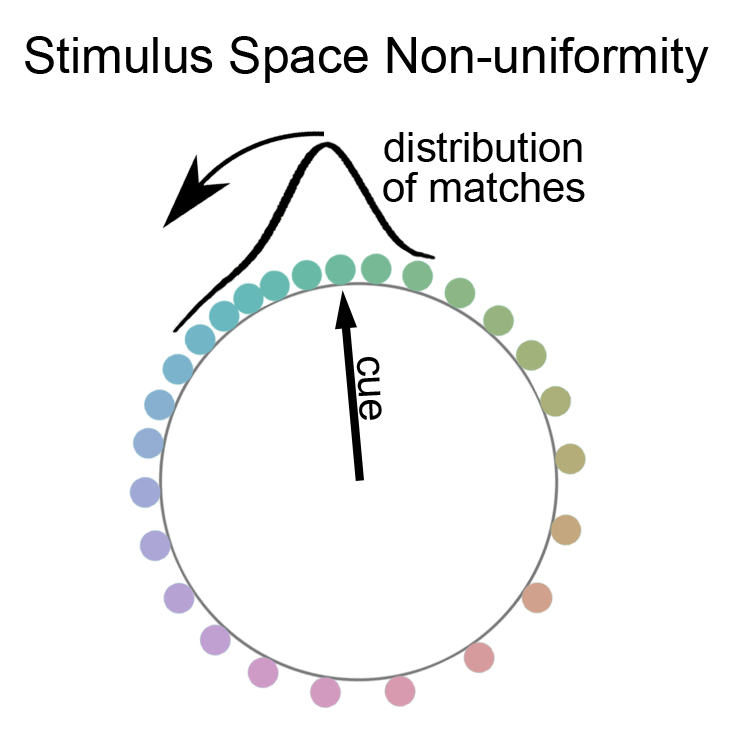
\includegraphics[height=4cm]{../Figures/working/F3_TCCModel/b.png}
         \label{fig:TCCCartoonB}
    \end{subfigure}
    
    \begin{subfigure}[t]{0.3\textwidth}
         \centering
         \caption{}
        \includesvg[pretex=\tiny, width=\textwidth]{../Figures/working/F3_TCCModel/F3_TCCModel_og_Output_fromPreProcessedData_postCombined_MixMod_polar_231110-022720.svg}
         \label{fig:TCCModel_og}
    \end{subfigure}
    \begin{subfigure}[t]{0.3\textwidth}
         \centering
         \caption{}
         \includesvg[pretex=\tiny, width=\textwidth]{../Figures/working/F3_TCCModel/TCCDemo_ssnu_fromModelOutput_MixMod_polar_231110-022647.svg}
         \label{fig:TCCModel_ssnu}
    \end{subfigure}

    \begin{subfigure}[t]{0.3\textwidth}
         \centering
         \caption{}
         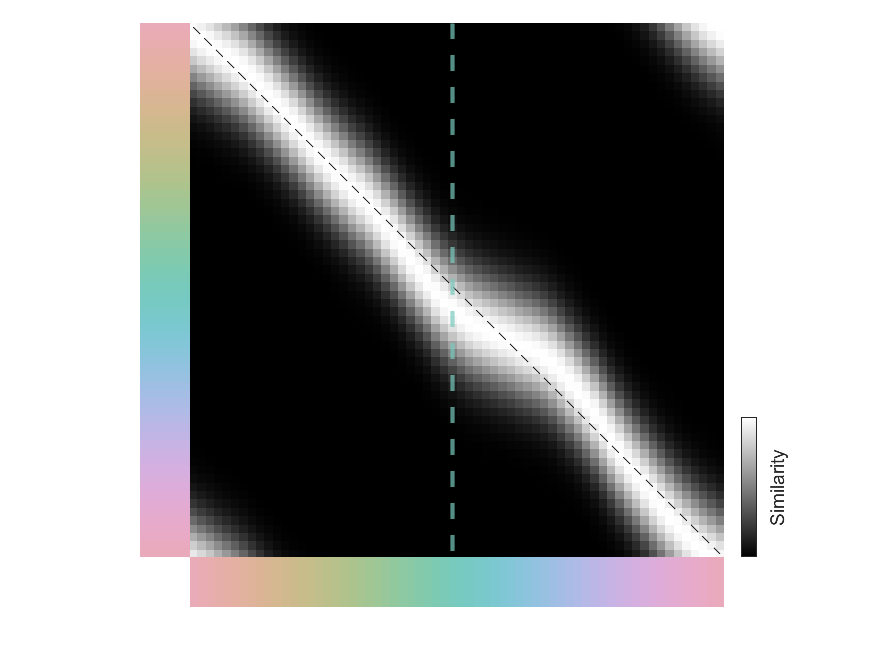
\includegraphics[width=\textwidth,trim={2cm 0.5cm 2 0},clip]{../Figures/working/F3_TCCModel/sm_og_231110-022722.png}
         \label{fig:TCCModel_og_sm}
    \end{subfigure}
    \begin{subfigure}[t]{0.3\textwidth}
         \centering
         \caption{}
         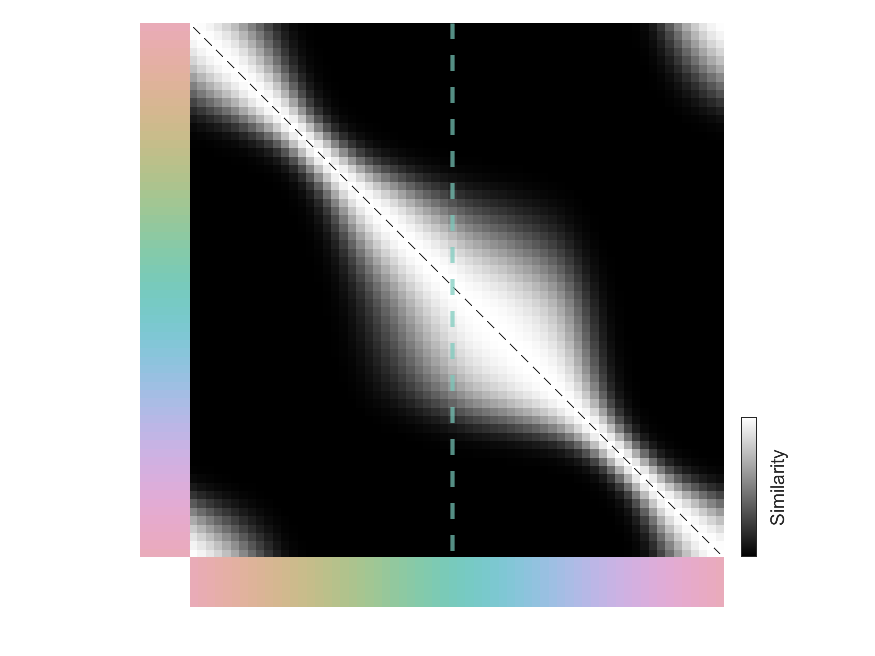
\includegraphics[width=\textwidth,trim={2cm 0.5cm 2 0},clip]{../Figures/working/F3_TCCModel/sm_ssnu_231110-022643.png}
         \label{fig:TCCModel_ssnu_sm}
    \end{subfigure}
    
    \begin{subfigure}[t]{0.3\textwidth}
         \centering
         \caption{}
         \includesvg[pretex=\ttiny, width=\textwidth]{../Figures/working/F3_TCCModel/og_SimilarityFunction_231110-183536.svg}
         \label{fig:TCCModel_og_sf}
    \end{subfigure}
    \begin{subfigure}[t]{0.3\textwidth}
         \centering
         \caption{}
         \includesvg[pretex=\ttiny, width=\textwidth]{../Figures/working/F3_TCCModel/ssnu_SimilarityFunction_231110-184008.svg}
         \label{fig:TCCModel_ssnu_sf}
    \end{subfigure}

    % \begin{subfigure}[t]{0.45\textwidth}
    %      \centering
    %      \caption{}
    %      \includesvg[pretex=\tiny, width=\textwidth]{../Figures/working/F3_TCCModel/sg_SimilarityFunction_230807-153339.svg}
    %      %\label{fig:JustBias_subset}
    % \end{subfigure}
    % \hfill
    % \begin{subfigure}[t]{0.45\textwidth}
    %      \centering
    %      \caption{}
    %      \includesvg[pretex=\tiny, width=\textwidth]{../Figures/working/F3_TCCModel/ssnu_SimilarityFunction_230731-150035}\llap{\raisebox{3cm}{\includesvg[pretex=\tiny, width=2.5cm]{../Figures/working/F6_ColSpace/combined_TCC-0att_fullremap-workspace_230510_behaviorally derived-colorspace_everySecond230818-114423.svg}}} 
    %      % h/t: https://tex.stackexchange.com/a/89778/169285 
    %      %\label{fig:JustColSpace_subset}
    % \end{subfigure}
        \caption{\textbf{Distinguishing between different sources of bias using TCC-MAT models: cognitive bias vs. non-uniformity of stimulus space.} Caption on following page.}
        \label{fig:TCCDemo}
\end{figure}

\begin{figure}[t]
  \contcaption{
  \emph{A and B.} Bias can be produced by two distinct mechanisms. \emph{A.} Where memory is encoded jointly as a continuous variable and a categorical variable, and decoding considers both, the resulting memory shall be biased towards the category center. 
  \emph{B.} Where the set of potential choices contains more plausible options on one side of the cue than on the other, as would be the case with a non-uniform stimulus-space, bias will be introduced towards the denser-populated part of space.
  \emph{C and D.} Simulated data using models implementing each of these mechanisms, analyzed using a mixture model, can result in identical representations. The dashed line in turquoise, at 180 degrees/stimulus number 32, will be used for demonstration purposes in the following panels.
  \emph{E and F.} Similarity matrices. These matrices represent the perceptual similarity between stimulus $i$ and stimulus $j$ (where the stimulus used as the cue is represented on the x-axis% TODO change if we change this
  and the stimulus used as the choice is represented on the y-axis.
  \emph{E.} Similarity matrix for a cognitive bias model. Here, asymmetric deviations away from the diagonal represent biases.
  \emph{F.} Similarity matrix for a stimulus-space non-uniformity model. Here, similarity is symmetric about the diagonal (stimulus $i$ is as similar to stimulus $j$, as stimulus $j$ is as similar to stimulus $i$).
  \emph{G and H.} Extracting single similarity functions from panels E and F we can see that both are biased towards higher stimuli. The cognitive bias model results in an offset gaussian, whereas the stimulus-space non-uniformity results in a skewed distribution.}% Continued caption
\end{figure}


The colors we used were defined by the International Commission on Illumination (CIE) to be approximately perceptually uniform. 
But it has long been recognized that there may be non-uniformities in the space \citep{stockman_colorimetry_2010}; some have argued that perceptual uniformity may be task-dependent or simply unattainable \citep{judd_ideal_1969}.

One might even suppose that if language influences color perception, as stipulated by the Sapir-Whorf hypothesis, then all color spaces generated by human observers could be shaped by language. 
Could the macaque consensus color categories be attributed not to a true cognitive category (\autoref{fig:TCCCartoonA}) but to unrecognized distortions in the presumed uniform space of colors (\autoref{fig:TCCCartoonB})?
Both explanations could introduce biases in the distribution of matches.

The difference in the two explanations can be understood by considering the relationship between two neighboring colors. 
For the cognitive-bias account, there is an asymmetry between the colors if there is a category center nearby.
The color further from the category center will be more likely mistaken for the color closer to the category center than the other way around. 
Whereas for the non-uniform color space, there is no asymmetry in mismatches between neighboring colors. 
These two explanations would produce different shaped distributions of matches: the cognitive bias would yield the same width distribution for all cues around the color circle, but the peak of the distribution would deviate from the cue to varying degrees depending on the proximity of the cue to the category center. 
A stimulus space non-uniformity, meanwhile, would yield an asymmetric distribution that varies in width depending on sampling density of the underlying uniform color space, with regions that are relatively densely sampled having broader distributions. 
We refer to the distributions of matches for a cue as its similarity function (hypothetical similarity functions shown in turquoise in \autoref{fig:TCCModel_og_sm,fig:TCCModel_ssnu_sm}).

To illustrate that the behavioral data could be explained by either a cognitive-bias account or a stimulus-space non-uniformity, we generated two sets of simulated data. 
One data set was generated with a simulation that used a uniform space and a bias arising from cognitive categories, and the other data set was generated with a simulation that used non-uniform sampling of an underlying uniform color space and no cognitive categories.
The data sets from both simulations gave rise to the same pattern of results when analyzed with a mixture model (\autoref{fig:TCCModel_og,fig:TCCModel_ssnu}).
These simulated data sets were chosen for illustration purposes because they correspond to the pattern of behavioral results (compare the simulated results with \autoref{fig:CombinedPolar). 
The simulations show that the results recovered by the mixture model could be explained by stimulus space non-uniformities without appeal to cognitive color categories. 

To tease apart the possible underlying causes of the behavioral results, we extended the Target Confusability Competition (TCC) generative model \citep{schurgin_psychophysical_2020} (see Methods). % Was it previously a generative model? I think technically not...
The standard implementation of the TCC model assumes the same similarity function for each color. 
The extended version developed presently, which we call TCC-v, allows the similarity function to vary as a function of color.
We introduce the concept of a similarity matrix, which captures the set of unique similarity functions for all colors in the space (the ``v'' in TCC-v is for ``vary'').
Let's consider three versions of the TCC-v model.
The simplest (“null”) model has the same two-parameter similarity function for each color, centered on the target color (this is conceptually equivalent to the standard TCC model).  The cognitive bias version specifies similarity functions for each color with peaks that can deviate from the target color (Figure 3e). The result is a similarity matrix that has a band of constant width along the inverse diagonal but deviates to one side at color-category locations in the color space. The stimulus-space non-uniformity version of the model, meanwhile, has a similarity function where the peak is fixed to the target color but where the angular distances between the colors can vary (Figure 3f). This results in a similarity matrix that is symmetric about the inverse diagonal, but which bulges at locations in the color space that are oversampled. The shape of the distribution of matches for a cue corresponding to the zero-crossing of the negative slope in the mixture model is indicated by the turquoise line in the cognitive bias and stimulus space non-uniformity versions of the TCC-v model. To recap, the similarity matrix in 3e is constructed using the same data as the polar plot in 3c; and the similarity matrix in 3f is constructed using the same data as the polar plot in 3d. These results show that different underlying mechanisms could explain the appearance of choice biases in color-matching tasks.

Next, we quantitatively compare the best fitting versions of each model to the behavioral data. To facilitate this comparison, we plot the behavioral data with a free-similarity version of the TCC-v model in which every cell in the similarity matrix is an independent model parameter (Figure 4a, 4b; the data for both panels are the same, centered on one or the other of the putative category centers recovered in the mixture model). The resulting matrix makes no assumptions about the underlying mechanisms that determine the similarity between any pair of stimuli. Now we can ask, are the data illustrated by the free similarity matrix better explained by the stimulus space non-uniformity model or the cognitive bias model? In other words, do the panels in Figure 4a,b show mirror symmetry with bulges about the diagonal (like Figure 3f) or asymmetry about the diagonal without bulges (like Figure 3e)? By visual inspection, the data are better explained by the stimulus space non-uniformity model, a conclusion affirmed by statistical tests. 

First, the stimulus space non-uniformity model provides a better fit of the data than the null model (Figure 4c). Second, the data are better explained by the stimulus-space non-uniformity model than the cognitive bias model (Figure 4d). These results strongly suggest that macaque monkeys do not have innate color categories. Again, if the macaque is an accurate model of the human, then the results imply that humans do not have innate color categories either. 

The data presented so far are for the four animals combined. The individual animals showed some idiosyncratic differences (SI Figure 4). By mixture-model analysis, one animal showed not only the two consensus choice biases but also a third bias, for pea green (Figure 5a). The free similarity matrix for the data from this animal shows an asymmetry about the diagonal at this location in the color space (Figure 5b), showing that this animal has a cognitive bias for pea-green in addition to the consensus biases driven by stimulus-space non-uniformities (free similarity matricies for all animals shown in SI Figure 5). These results show that macaque monkeys have the potential to form cognitive color biases, and that the TCC-v model can recover them. The existence of cognitive biases in individual animals is consistent with prior work that observed different patterns of color-matching behavior in two animals using the continuous-matching task that likely reinforces idiosyncratic acquired biases \citep{panichello_error-correcting_2019}.


\begin{figure}
    \centering
    \begin{subfigure}[t]{0.33\textwidth}
         \centering
         \caption{}
         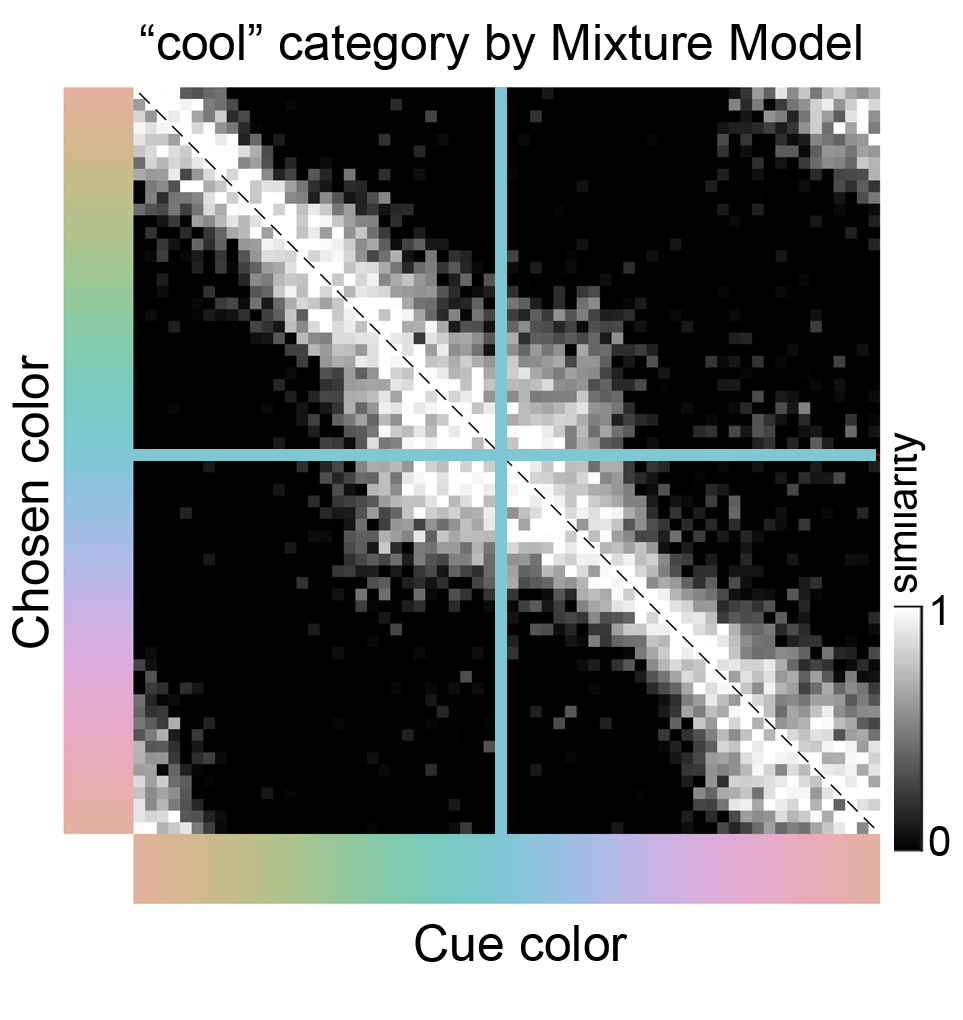
\includegraphics[height=5cm]{../Figures/working/F4_TCCResults/a.png}         \label{fig:SimilarityMatrixCombined_Cool}
    \end{subfigure}
    \hfill
    \begin{subfigure}[t]{0.33\textwidth}
         \centering
         \caption{}
         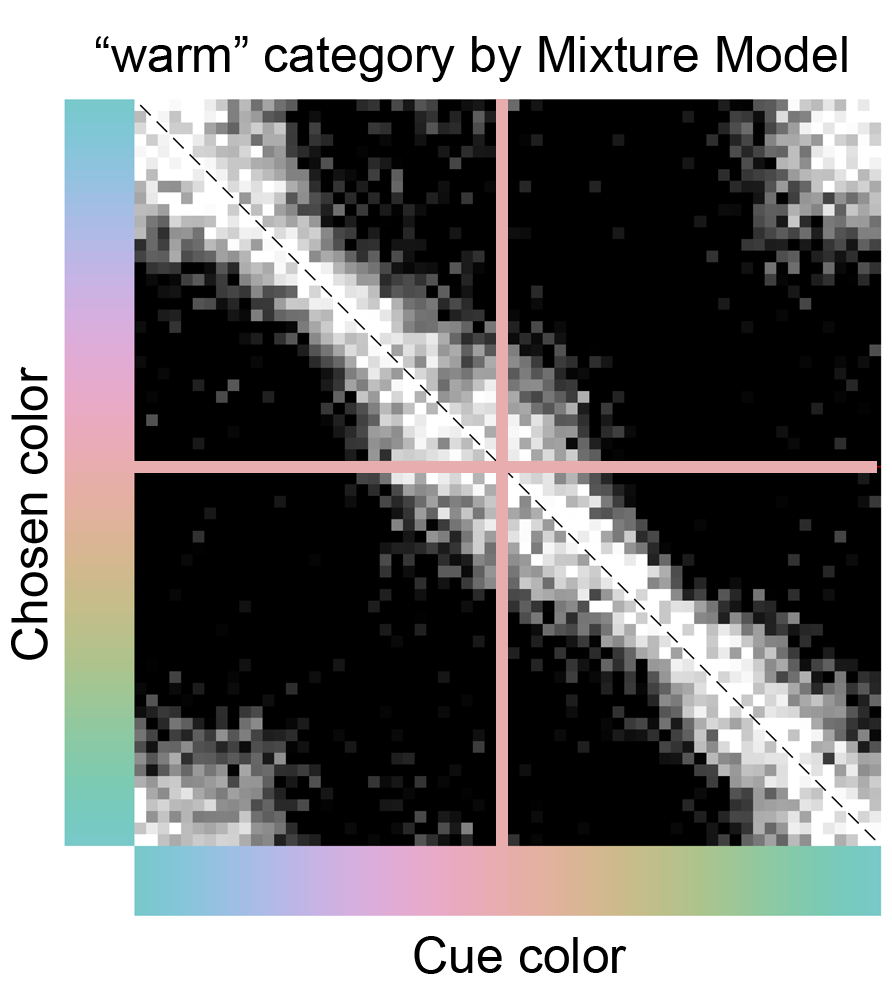
\includegraphics[height=5cm]{../Figures/working/F4_TCCResults/b.png}   \label{fig:SimilarityMatrixCombined_Warm}
    \end{subfigure}
    \hfill
       \begin{subfigure}[t]{0.29\textwidth}
         \centering
         \caption{}
         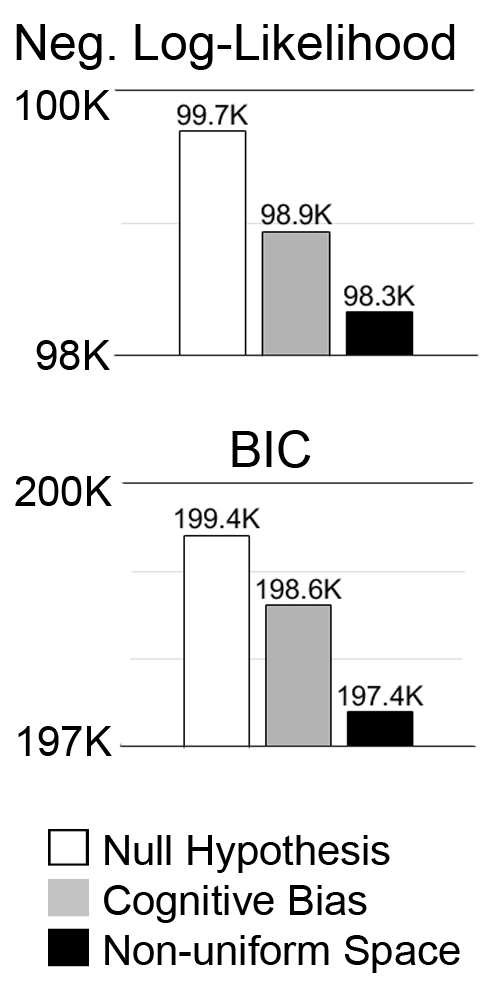
\includegraphics[height=5cm]{../Figures/working/F4_TCCResults/c.png}   
         \label{fig:Combined-ModelFitAnalysis}
    \end{subfigure}
    \caption{\textbf{Model comparison.}
    \emph{A and B.} "Free similarity" model similarity matrices for combined data, centered on the "cool" and the "warm" attractor points. 
    In this type of model, no particular relationship is pre-supposed between any of the stimuli. 
    If the underlying mechanism for the attractor points were cognitive bias, we would see an asymmetry around the diagonal (as in \autoref{fig:TCCModel_og_sm}), whereas if the underlying mechanism were stimulus-space non-uniformity we would see bulges away from the diagonal at the attractor points which would be symmetric about the diagonal (as in \autoref{fig:TCCModel_ssnu_sm}).
    \emph{C.} Quantitative comparison between models. Negative log likelihood of a null model (no bias), the cognitive bias model, and a stimulus-space non-uniformity model. Lower negative log likelihoods indicate a better fit to the data. BIC values allow us to compare performance taking into account the number of model parameters and the number of trials, and also provide a unit by which the confidence of model superiority can be judged. Lower BIC values indicate a better fit to the data. BIC differences of between 6 and 10 are generally interpreted as strong evidence that one model is better than another; here we see a BIC difference of roughly 1200.
    } 
    \label{fig:TCCOutput}
\end{figure}

\begin{figure}
    \centering
    \begin{subfigure}[t]{0.49\textwidth}
         \centering
         \caption{}
         \includesvg[pretex=\tiny, width=\textwidth]{../Figures/working/SI/SI1_IndiMM/210517--211108_Castor_data_fromModelOutput_MixMod_polar_231105-230855.svg}
         \label{fig:CastorMM}
    \end{subfigure}
    \hfill
    \begin{subfigure}[t]{0.49\textwidth}
         \centering
         \caption{}
         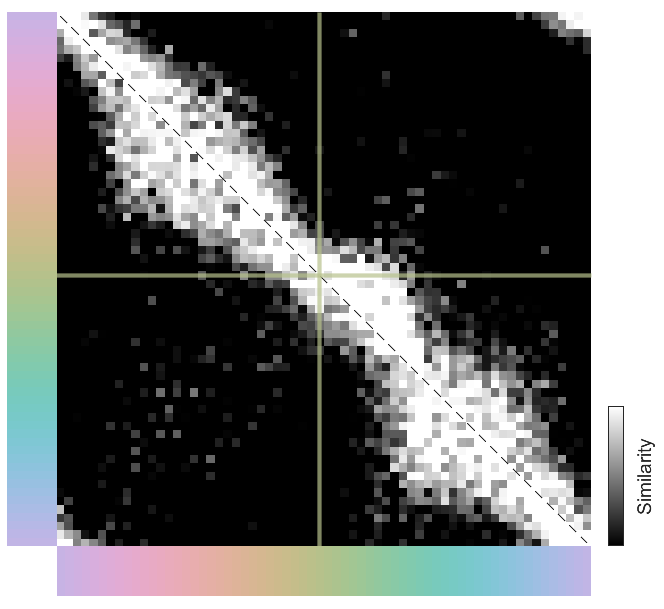
\includegraphics[width=\textwidth]{../Figures/working/F5_CastorCogBias/sm_18_231110-202911.png}
         \label{fig:Castor-FreeSimilarity}
    \end{subfigure}
    \caption{\textbf{Idiosyncratic cognitive bias at the individual level.} 
    \emph{A.} Mixture model for animal CA. In addition to the shared "warm" and "cool" attractor points, another attractor point is recovered in the yellow/green region.
    \emph{B.} TCC-MAT modeling reveals an asymmetry indicative of a cognitive bias which is shifting higher hue angles to lower values.}
    \label{fig:IndiDataCogBias}
\end{figure}

\begin{figure}
    \centering
    \begin{subfigure}[t]{0.3\textwidth}
         \centering
         \caption{}
         \includesvg[pretex=\tiny, width=\textwidth]{../Figures/working/F6_ColSpace/colorspace_everySecond230818-114428.svg}
         \label{fig:CIELUV}
    \end{subfigure}
    \hfill
    \begin{subfigure}[t]{0.3\textwidth}
         \centering
         \caption{}
         \includesvg[pretex=\tiny, width=\textwidth]{../Figures/working/F6_ColSpace/combined_TCC-0att_fullremap-workspace_230510_behaviorally-derived-colorspace_everySecond230818-114423.svg}
         \label{fig:MACBEHspace}
    \end{subfigure}
    \hfill
    \begin{subfigure}[t]{0.3\textwidth}
         \centering
         \caption{}
         \includesvg[pretex=\tiny, width=\textwidth]{../Figures/working/F6_ColSpace/newEqualSampling230818-170747.svg}
         \label{fig:UniformStimsInCIELUV}
    \end{subfigure}
           \caption{\textbf{A behaviorally derived colorspace.} 
           \emph{A.} Stimuli in CIELUV. 
           \emph{B.} Stimuli in behaviorally derived space, extracted from the TCC-MAT stimulus-space non-uniformity model for combined data. 
           \emph{C.} Stimuli sampled uniformly in behaviorally derived space, projected back into CIELUV.}
        \label{fig:MACBEHcolorspace}
    
\end{figure}


\paragraph{A perceptually uniform color space unconfounded by language}

The behavioral data in macaques provide a rare opportunity to reconstruct a perceptually uniform color space unconfounded by language.
We computed, empirically, a transformed color space such that the macaques would, on average, show no choice bias. 
We refer to this space as the Macaque Uniform Color Space (MUCS). 
When colors evenly sampled from the purportedly uniform CIELUV space (Figure 6a) are plotted within this macaque-derived uniform color space, colors are bunched around the teal part of the space, and to a lesser extent, around the peach-colored part of the space (Figure 6b). 
We can then take colors sampled at uniform intervals in MUCS and project them into CIELUV (Figure 6c). This arrangement shows relative bunching around the yellows and purples, which correspond to the colors of the poles of the S-cone-opponent axes. 
These results are consistent with those obtained in human infants \citep{skelton_biological_2017} and adults \citep{bae_why_2015,panichello_error-correcting_2019} showing repeller points aligned with the poles of the S-cone axis (the only two repeller points identified in the macaque monkeys aligned with the poles of the S-cone axis, see the zero crossings of the positive slope in Figure 1d,e), and suggest a mechanism by which the non-uniformities emerge in CIELUV. 
The CIELUV colors were defined at threshold, whereas the color-matching experiments were conducted suprathreshold. 
The results in Figure 6c suggest that supra-threshold discrimination for colors that modulate the S-cone axis is higher than at threshold, suggestive of an amplification of subcortical S-cone signals \citep{RN655}. 

The present results are consistent with the idea that color ordering and the capacity to form color categories is innate, but not color categories themselves. 
If color categories are not innate, where do they come from? We wonder whether color categories reflect the behavioral relevance of colors in the world; the relevance of things is partially culturally determined, introducing a role for language in shaping consensus color categories. 
Given that color categories can be learned, as evident in at least one macaque in our study (Figure 5) and two macaques in another study \citep{panichello_error-correcting_2019}, the introduction of language provides a mechanism by which cultures can acquire consensus color categories. 
For example, the parts of scenes labeled as objects by human observers are more likely to be warm colored while backgrounds are more likely to be cool colored \citep{rosenthal_color_2018}, and these statistics predict universal patterns in color naming \citep{gibson_color_2017}. 
We speculate that the choice biases in humans, which include at least double the number of consensus choice biases in monkeys, likely reflect cognitive biases, and that these cognitive biases achieve consensus through shared behavioral relevance and communication \citep{RN18511,RN18514,RN18602}. 
